% !TEX TS-program = Xelatex
% !TEX encoding = UTF-8 Unicode

\documentclass[UTF8]{ctexart}
\usepackage{amsmath}
\usepackage[bottom]{footmisc}
\usepackage{geometry}
\usepackage{hyperref}
\usepackage{graphicx}
\usepackage{figsize}
\usepackage[separate-uncertainty = true,per-mode=symbol]{siunitx}
\usepackage{tabu}
\usepackage{wasysym}
\geometry{left=0.7in,right=0.7in,bottom=0.7in,top=0.7in}

\title{实验二十九:虚拟仪器}
\author{朱寅杰 1600017721}
\date{2018年5月25日}

\begin{document}
\maketitle
\paragraph{思考题}
虚拟仪器系统只对外保留了传感器和发生器的接口,而把中间的测量和逻辑过程全部放在计算机内完成。而传统仪器的所有测量值传递和中间运算和逻辑过程都是内嵌在外设仪器里的,最多只能插个U盘把结果拷出来。

比如富朗克-赫兹实验,我们可以直接让电脑程序控制(可能经过一个放大器)加扫描电压,然后电流值也经过一个放大转换直接接到板子上读进电脑,这样编好程序以后一切都是自动完成,可以直接拿到最后的伏安曲线图。

不同时直接测量待测电阻和标准电阻上电压的原因主要还是共接地问题,两个电压传感器要和产生电平的电源共地,所以肯定有一个数要把两个电压作差得到。实验的误差主要还是来自于接收电压信号的板子自身的精度。这个板子也就是一个做数模转换的,也是和普通数字万用表一样有允差,最后一位数会跳来跳去的。要说算误差的话就查一下板子的说明书,看看允差多少,再和拟合统计评估出来的误差合成一下就行了。

画二极管伏安特性曲线的时候要注意合理控制正向和反向的扫描范围和曲线上各段采样的密度。在电流变化较平坦的段落可以少采一些,在曲线拐弯陡峭处要多采一些。

\begin{figure}
\centering
\SetFigLayout{2}{2}
\subfigure[对$R_1$阻值的测量。拟合得出阻值为\SI{50.5679}{\ohm}。]{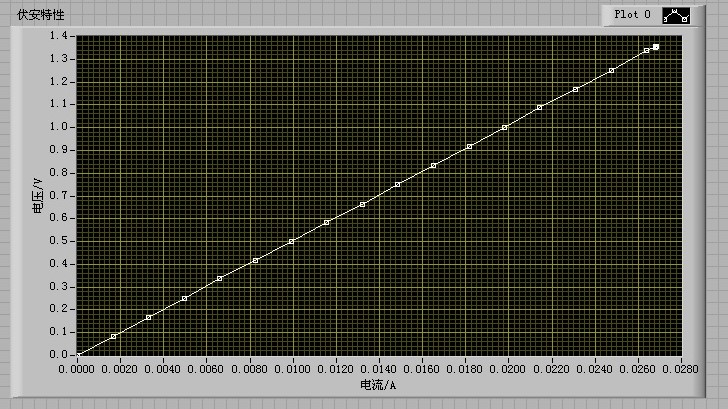
\includegraphics[width=0.49\linewidth]{R1.jpg}} \hfill
\subfigure[对$R_2$阻值的测量。拟合得出阻值为\SI{994.153}{\ohm}。]{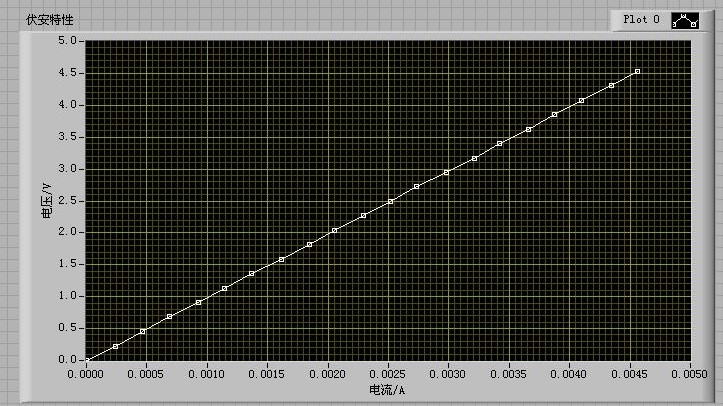
\includegraphics[width=0.49\linewidth]{R2.jpg}} \\
\subfigure[稳压二极管的伏安特性。正向电流达到\SI{5}{mA}时静态阻值约为\SI{155}{\ohm},反向电流达到\SI{5}{\mA}时候静态阻值约为\SI{1110}{\ohm}。]{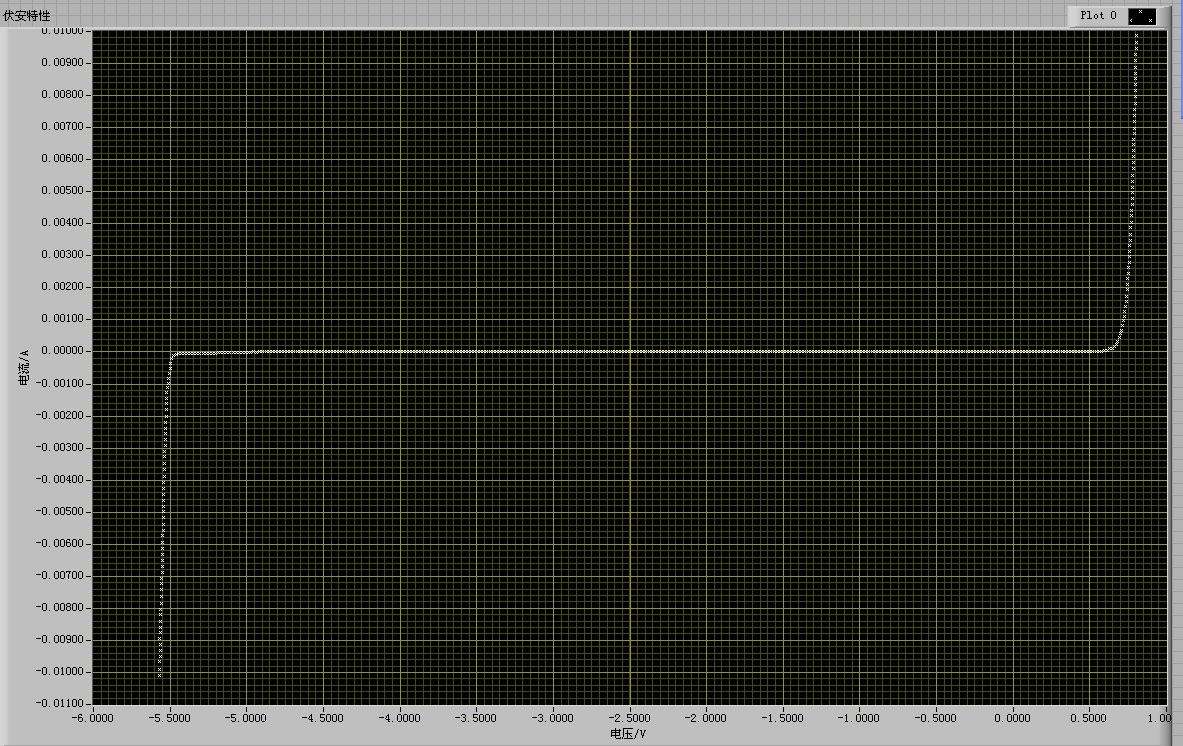
\includegraphics[width=\linewidth]{erjiguan.jpg}} \\
\end{figure}

\end{document} 